\documentclass[12pt]{article}

\usepackage{geometry}
\geometry{a4paper,left=2.5cm,right=2.5cm,top=2.5cm,bottom=2.5cm}

\usepackage{graphicx}
\usepackage{amsmath}
\usepackage{booktabs}
\usepackage{longtable}
\usepackage{hyperref}
\usepackage{indentfirst} 
\usepackage[numbers,sort&compress]{natbib}

\title{Development of a Machine Learning-Based Mortality Risk Prediction Model Integrating Clinical Indicators for Patients with Heart Failure}
\author{Liang Yanhua}
\date{10 July 2026}

\begin{document}

\maketitle

\begin{abstract}
Heart failure (HF) is a complex clinical syndrome characterized by structural and functional cardiac abnormalities and is associated with substantial morbidity and mortality worldwide. Owing to the considerable heterogeneity in disease progression among patients, accurate identification of individuals at high risk of death is essential for early risk stratification, optimized clinical management, and improved prognosis.
This study aimed to develop an individualized mortality risk prediction model for patients with heart failure by integrating conventional statistical analyses with machine learning algorithms using routinely available clinical indicators.
The Heart Failure Clinical Records Dataset was used as the study cohort. Data preprocessing included descriptive statistical analysis, missing-value assessment, outlier detection using the interquartile range (IQR) method, Winsorization, and feature standardization. Pearson correlation analysis, the Mann–Whitney U test, and Random Forest feature importance analysis were jointly employed to identify clinically relevant predictors of mortality. Four predictive models—Logistic Regression (LR), Random Forest (RF), eXtreme Gradient Boosting (XGBoost), and Multilayer Perceptron (MLP)—were developed and evaluated. Model performance was assessed using Accuracy, Precision, Recall, F1-score, and the area under the receiver operating characteristic curve (ROC-AUC).
Three clinical variables, namely follow-up time (time), serum creatinine, and ejection fraction, were consistently identified as the most influential predictors of mortality. Among the four machine learning models, the Random Forest model achieved the best overall predictive performance, yielding the highest ROC-AUC of 0.883. Furthermore, the optimized Random Forest model successfully generated individualized mortality probabilities. In a representative simulated patient, the predicted probability of mortality reached 84.5%, demonstrating the model's capability for personalized risk estimation.
This study developed a machine learning-based mortality risk prediction model by integrating multiple clinical indicators with statistical feature selection methods. The proposed model enables individualized probability-based mortality assessment and may serve as a valuable decision-support tool for clinical risk stratification and personalized management of patients with heart failure.

\noindent\textbf{Keywords:}
Heart failure; Machine learning; Random Forest; Mortality risk prediction; Clinical risk factors; Artificial intelligence; Clinical prediction model
\end{abstract}



\section{Introducion}

Heart failure (HF) is a complex and highly heterogeneous clinical syndrome characterized by structural and/or functional abnormalities of the heart that impair ventricular filling or ejection, ultimately leading to inadequate systemic perfusion. The condition commonly results from a variety of cardiovascular disorders, including coronary artery disease, hypertension, cardiomyopathy, and valvular heart disease. As the disease progresses, pathological changes such as ventricular remodeling, impaired myocardial contractility, and reduced cardiac output may occur, eventually resulting in severe cardiac dysfunction and adverse clinical outcomes. Despite continuous advances in pharmacological and device-based therapies, heart failure remains one of the leading causes of hospitalization and mortality worldwide.\cite{McDonagh2021,Heidenreich2022}

With the rapid aging of the global population and the increasing prevalence of cardiovascular diseases, heart failure has become a major public health challenge. Although substantial improvements have been achieved in the diagnosis and management of HF, patients continue to experience high rates of mortality and recurrent hospitalization. Consequently, accurate prediction of patient prognosis and early identification of individuals at high risk of adverse outcomes have become essential components of contemporary heart failure management. Early risk stratification facilitates individualized treatment planning, optimizes the allocation of healthcare resources, and may ultimately improve long-term clinical outcomes.\cite{Savarese2023}

Current clinical risk assessment for patients with heart failure primarily relies on demographic characteristics, cardiac functional parameters, laboratory findings, and medical history. Conventional indicators such as left ventricular ejection fraction (LVEF) and serum creatinine have been widely recognized as important prognostic biomarkers because they reflect cardiac systolic function and renal function, respectively. However, heart failure is a multifactorial disease in which patient outcomes are influenced by complex interactions among numerous physiological and pathological factors. Therefore, reliance on a single clinical indicator or conventional statistical models based on linear assumptions may be insufficient to accurately characterize disease severity and predict patient prognosis.

The rapid development of healthcare informatics has generated an unprecedented volume of clinical data, providing new opportunities for data-driven disease prediction. In recent years, machine learning (ML) techniques have attracted increasing attention in medical research because of their ability to analyze high-dimensional data, identify complex nonlinear patterns, and automatically discover hidden relationships among clinical variables. Compared with traditional statistical approaches, machine learning algorithms can substantially improve predictive performance while simultaneously providing quantitative assessments of feature importance, thereby facilitating the identification of clinically meaningful prognostic factors and supporting personalized risk assessment.\cite{Rajkomar2019,Esteva2019}

Among various machine learning algorithms, Random Forest (RF) has demonstrated considerable advantages in clinical prediction tasks. As an ensemble learning method, Random Forest constructs multiple decision trees and integrates their predictions to improve model robustness and reduce overfitting. In addition, the algorithm provides measures of feature importance, which enhance model interpretability and facilitate the identification of clinically relevant risk factors. Owing to its capability to capture complex nonlinear relationships among variables, Random Forest has been successfully applied to numerous medical prediction problems and has shown particular promise in prognostic modeling for chronic diseases.\cite{Breiman2001}

Against this background, the present study aimed to develop an individualized mortality risk prediction model for patients with heart failure by integrating statistical feature selection methods with multiple machine learning algorithms. First, comprehensive data preprocessing was performed, including data quality assessment, outlier detection, and feature standardization. Subsequently, Pearson correlation analysis, the Mann–Whitney U test, and Random Forest feature importance analysis were jointly employed to identify the most informative clinical predictors associated with mortality. Finally, four predictive models—Logistic Regression (LR), Random Forest (RF), eXtreme Gradient Boosting (XGBoost), and Multilayer Perceptron (MLP)—were established and systematically compared using multiple evaluation metrics to determine the optimal prediction model.

The specific objectives of this study were as follows:

    1.To identify key clinical variables associated with mortality in patients with heart failure through comprehensive statistical and machine learning analyses.
    
    2.To develop and compare multiple machine learning models for mortality risk prediction and determine the algorithm with the best predictive performance.
    
    3.To generate individualized mortality probabilities using the optimal prediction model, thereby providing quantitative support for clinical risk stratification and personalized decision-making.

Overall, this study proposes a data-driven framework that integrates routinely available clinical indicators with machine learning techniques for individualized mortality risk prediction in patients with heart failure. The proposed framework has the potential to support precision medicine by improving clinical risk assessment and facilitating personalized management strategies.
\begin{figure}[htbp]
    \centering
    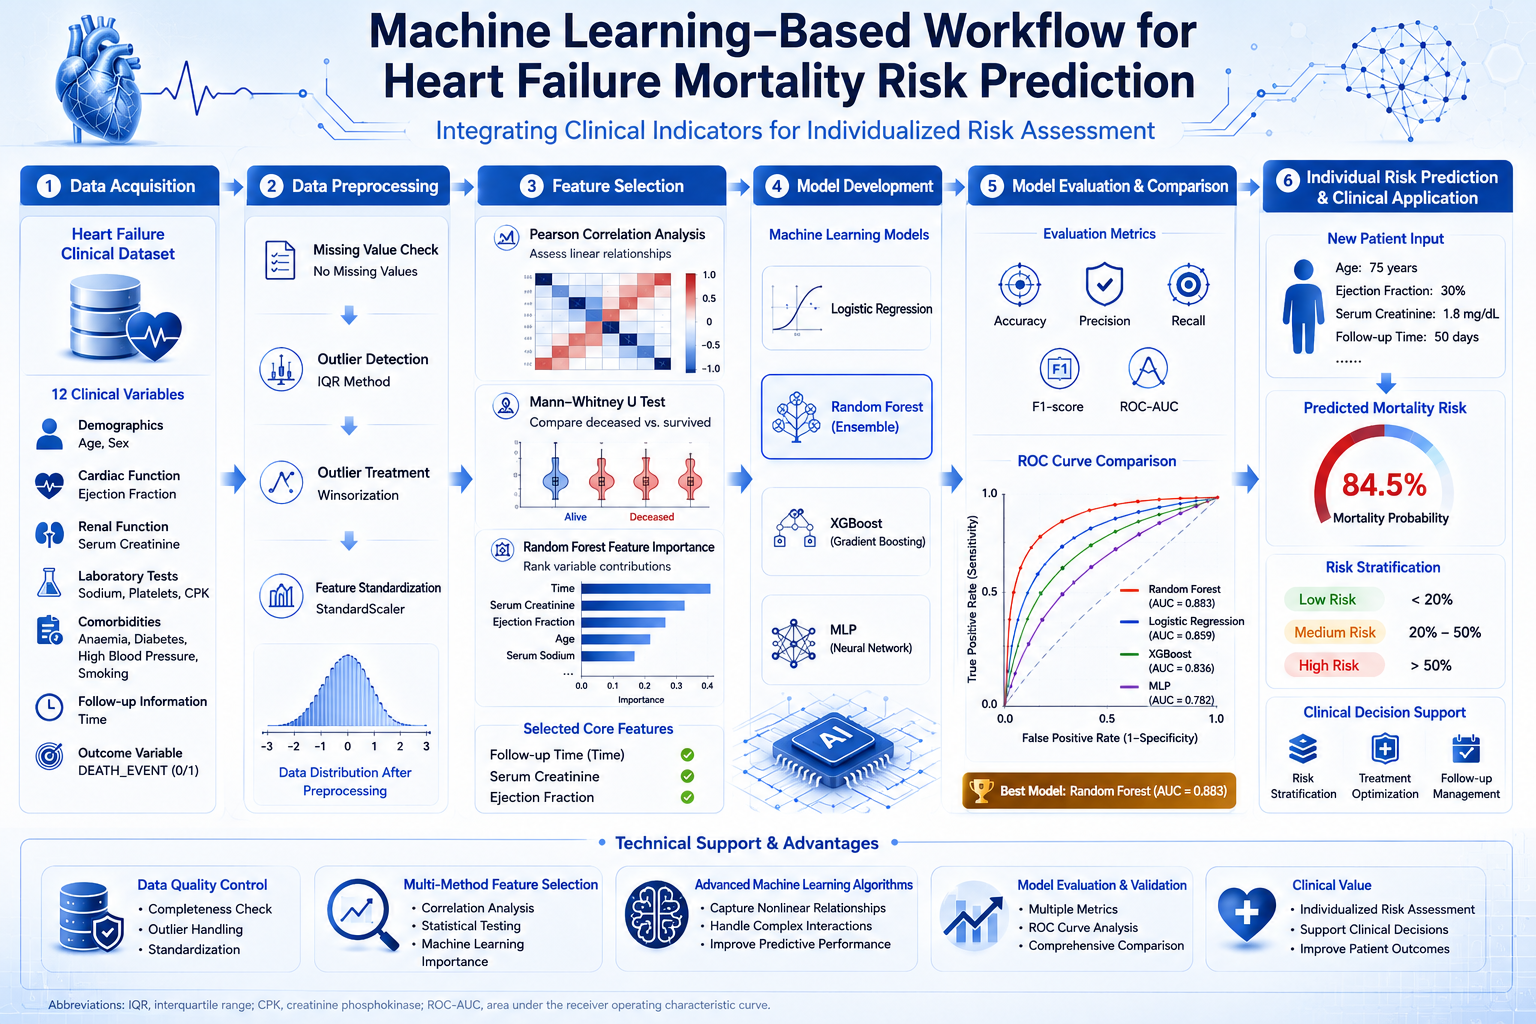
\includegraphics[width=0.5\linewidth]{ChatGPT Image 2026年7月10日 15_20_21.png}
    \label{fig:placeholder}
\end{figure}

\section{Methods}

\subsection{Data Source}

This study was conducted using theHeart Failure Clinical Records Dataset, a publicly available dataset containing demographic characteristics, clinical variables, laboratory measurements, and follow-up outcomes of patients diagnosed with heart failure. The primary outcome variable was DEATH\_EVENT, where a value of 0 indicated survival during the follow-up period and 1 represented death.

The dataset included twelve predictor variables: age, anaemia, creatinine\_phosphokinase, diabetes, ejection\_fractioz, high\_blood\_pressure, platelets, serum\_creatinine, serum\_sodium, sex, smoking, and time. These variables comprehensively describe patients' demographic characteristics, comorbidities, laboratory findings, cardiac function, renal function, and follow-up information, thereby providing a comprehensive representation of the clinical status of patients with heart failure.

The objective of this study was to predict mortality during the follow-up period by exploring the relationships between routinely collected clinical indicators and patient outcomes. A machine learning-based mortality risk prediction model was subsequently developed to estimate individualized probabilities of death. 

\subsection{Data Preprocessing}

Clinical datasets often exhibit inconsistencies arising from heterogeneous measurement scales, extreme observations, and variable data quality. Therefore, comprehensive data preprocessing was performed before model development to improve data reliability, enhance model stability, and ensure robust predictive performance.

\subsubsection{Descriptive Statistical Analysis}

Descriptive statistical analysis was first conducted to characterize the distribution of all clinical variables. Continuous variables were summarized using the mean, standard deviation (SD), minimum, quartiles, and maximum, providing an overall overview of the data distribution.

This preliminary analysis facilitated the identification of variable ranges and distributional characteristics, thereby providing a foundation for subsequent data quality assessment and preprocessing procedures. 

\subsubsection{Missing Value Assessment}

Missing values may adversely affect model training and predictive performance. Therefore, data completeness was evaluated by calculating the number of missing observations for each variable.

The assessment demonstrated that the dataset contained no missing values across all variables. Consequently, no imputation procedures were required prior to model development. 

\subsubsection{Outlier Detection and Treatment}

Extreme observations may substantially influence model training and reduce prediction accuracy. To identify potential outliers, the interquartile range (IQR) method was adopted.

The IQR was calculated as
\[
IQR = Q_3 - Q_1
\]
represent the first and third quartiles, respectively. Observations falling below
\[
Q_1 - 1.5 \times IQR
\]
above
\[
Q_3 + 1.5 \times IQR
\]
were considered potential outliers.

Outlier detection indicated that several variables, including creatinine\_phosphokinase, ejection\_fraction, platelets, serum\_creatinine, and serum\_sodium, contained extreme values.

Rather than removing these observations, Winsorization was applied to limit extreme values within acceptable boundaries while preserving the overall distribution of the original data. This approach effectively reduced the influence of extreme observations without discarding clinically meaningful information that might reflect genuine pathological conditions. 

\subsubsection{Data Standardization}

Clinical variables frequently differ substantially in measurement units and numerical scales. For example, age is generally measured within a range of several decades, whereas platelet counts may exceed hundreds of thousands. Such differences may bias optimization during model training, particularly for algorithms sensitive to feature scaling.

To eliminate the influence of variable magnitude, all continuous variables were standardized using the StandardScaler algorithm. Standardization transforms each feature according to
\[
X'=\frac{X-\mu}{\sigma}
\]
Following standardization, all continuous variables were transformed to comparable numerical scales, thereby improving optimization stability and facilitating fair comparisons among different machine learning algorithms. Although tree-based algorithms such as Random Forest are generally insensitive to feature scaling, standardization was applied consistently to ensure uniform preprocessing across all predictive models. 

 

\subsection{Feature Selection}

To identify the most informative clinical variables associated with mortality in patients with heart failure, a comprehensive feature selection strategy combining statistical analysis and machine learning techniques was adopted. Specifically, Pearson correlation analysis, the Mann–Whitney U test, and Random Forest feature importance analysis were jointly employed. By integrating these complementary approaches, feature relevance was evaluated from three perspectives: linear association with the outcome, statistical differences between patient groups, and contribution to predictive model performance. 

\subsubsection{Pearson Correlation Analysis}

Pearson correlation analysis was first performed to quantify the linear relationship between each clinical variable and the mortality outcome. The Pearson correlation coefficient (rrr) ranges from −1 to 1, where values approaching 1 indicate a strong positive correlation, values approaching −1 indicate a strong negative correlation, and values near 0 suggest little or no linear association.

This analysis provided an initial assessment of variables that were potentially associated with mortality while also revealing possible correlations among clinical predictors. 

\subsubsection{Mann–Whitney U Test}

Because several clinical variables did not satisfy the assumption of normality, the non-parametric Mann–Whitney U test was performed to compare differences in variable distributions between the deceased and surviving patient groups.

Statistical significance was determined using a significance threshold of P < 0.05. Variables with statistically significant differences between the two groups were considered potential predictors of mortality and were retained for further evaluation. 

\subsubsection{Random Forest Feature Importance Analysis}

To further evaluate the contribution of each predictor to mortality prediction, feature importance was calculated using the Random Forest algorithm.

Random Forest estimates feature importance by quantifying the contribution of each variable to node splitting across multiple decision trees. Compared with conventional statistical analyses, this approach better captures nonlinear relationships and complex interactions among variables, thereby providing a more comprehensive assessment of predictor relevance.

The final selection of core clinical predictors was based on the combined evidence from:

\begin{itemize}
    \item Pearson correlation analysis; 
    \item Mann–Whitney U testing; and 
    \item Random Forest feature importance ranking. 
\end{itemize}
Variables consistently identified as important by all three approaches were regarded as the most clinically informative predictors and were subsequently used for model construction. 

\subsection{Machine Learning Model Construction}

To compare the predictive performance of different machine learning algorithms for mortality prediction in patients with heart failure, four supervised learning models were developed:

\begin{itemize}
    \item Logistic Regression (LR); 
    \item Random Forest (RF); 
    \item eXtreme Gradient Boosting (XGBoost); and 
    \item Multilayer Perceptron (MLP). 
\end{itemize}
These algorithms represent both conventional statistical learning methods and modern ensemble and neural network approaches, allowing a comprehensive comparison of predictive capability across different modeling strategies. 

\subsubsection{Logistic Regression}

Logistic Regression (LR) is a classical binary classification algorithm that estimates the probability of an outcome by modeling the relationship between predictor variables and the log-odds of the target event.

Because of its straightforward interpretation and widespread clinical application, Logistic Regression was included as the baseline model for performance comparison. 

\subsubsection{Random Forest}

Random Forest (RF) is an ensemble learning algorithm that constructs multiple decision trees using bootstrap sampling and aggregates their predictions through a majority voting mechanism.

Compared with a single decision tree, Random Forest offers several advantages, including improved predictive stability, effective modeling of nonlinear relationships, and automatic estimation of feature importance. These characteristics make it particularly suitable for clinical prediction tasks involving multiple interacting variables. 

\subsubsection{eXtreme Gradient Boosting}

eXtreme Gradient Boosting (XGBoost) is a gradient boosting ensemble algorithm that sequentially optimizes weak learners to minimize prediction errors.

By iteratively improving model performance, XGBoost effectively captures complex nonlinear associations among clinical variables. The algorithm was therefore included to compare its predictive capability with that of the other machine learning models evaluated in this study. 

\subsubsection{Multilayer Perceptron}

The Multilayer Perceptron (MLP) is a feed-forward artificial neural network consisting of multiple hidden layers that learn nonlinear mappings between input features and target outcomes.

In this study, the MLP model was employed as a representative deep learning approach to compare the performance of neural network-based methods with conventional machine learning algorithms for mortality prediction in heart failure. 

\subsection{Model Evaluation}

To comprehensively evaluate model performance, five widely used classification metrics were adopted: Accuracy, Precision, Recall, F1-score, and the area under the receiver operating characteristic curve (ROC-AUC). 

\subsubsection{Accuracy}

Accuracy represents the proportion of correctly classified samples among all observations and provides an overall measure of classification performance.

\[\mathrm{Accuracy=\frac{TP+TN}{TP+TN+FP+FN}}\]

\subsubsection{Precision}

Precision is defined as the proportion of correctly predicted positive cases among all samples predicted as positive. This metric reflects the reliability of positive predictions generated by the model.

\[\mathrm{Precision=\frac{TP}{TP+FP}}
\]

\subsubsection{Recall}

Recall represents the proportion of actual positive cases that are correctly identified by the model and evaluates its ability to detect high-risk patients.

\[\mathrm{Recall=\frac{TP}{TP+FN}}\]

\subsubsection{F1-score}

The F1-score is the harmonic mean of Precision and Recall and provides a balanced evaluation of classification performance, particularly for datasets with class imbalance.

\[\mathrm{F1=2×\frac{Precision×Recall}{Precision+Recall}}\]



\subsubsection{ROC-AUC}

The receiver operating characteristic (ROC) curve illustrates the trade-off between sensitivity and specificity across different classification thresholds.

The area under the ROC curve (AUC) quantifies the model's overall ability to discriminate between patients who experienced mortality and those who survived. Higher AUC values indicate superior discriminative performance and greater predictive accuracy. 

\subsection{Individualized Mortality Risk Prediction}

Following comparative evaluation of all predictive models, the best-performing algorithm was further applied to estimate individualized mortality risk.

By inputting routinely available clinical variables, including age, ejection fraction, serum creatinine, and follow-up time, the optimized model generated the probability of mortality for each patient. Unlike conventional binary classification models that provide only categorical predictions (survival or death), the proposed approach outputs continuous probability estimates, enabling quantitative assessment of individual mortality risk.

This probability-based prediction framework offers a more intuitive representation of patient prognosis and may provide valuable support for clinical risk stratification and individualized decision-making in heart failure management.

\section{Results}

\subsection{Clinical Characteristics of the Dataset}

Before model development, descriptive statistical analysis was performed to characterize the distribution of clinical variables in the Heart Failure Clinical Records Dataset and to provide a foundation for subsequent feature selection and predictive modeling.

The descriptive statistics demonstrated considerable variability among continuous clinical variables. Patient age ranged from 40 to 95 years, with a mean of 60.83 years. The mean left ventricular ejection fraction (LVEF) was 38.08\%, indicating impaired cardiac systolic function in a substantial proportion of patients. The mean serum creatinine level was 1.394 mg/dL, whereas the maximum value reached 9.4 mg/dL, suggesting severe renal dysfunction in a subset of patients. In addition, platelet count and creatinine phosphokinase (CPK) exhibited substantial variability, reflecting marked inter-individual heterogeneity within the study population.

Subsequently, data completeness was assessed. No missing values were identified for any variable, indicating that the dataset was complete and suitable for subsequent analyses without the need for data imputation.

Potential outliers were then detected using the interquartile range (IQR) method. Extreme observations were identified in creatinine phosphokinase, ejection fraction, platelet count, serum creatinine, and serum sodium. Because these observations were considered likely to represent genuine clinical conditions rather than data entry errors, Winsorization was applied to reduce the influence of extreme values while preserving the overall distribution of the original data.

Finally, continuous variables were standardized using the StandardScaler algorithm to minimize the influence of different measurement scales and improve model training stability.

Overall, these preprocessing procedures generated a high-quality dataset that provided a reliable basis for subsequent statistical analyses and machine learning model development. 

\subsection{Feature Selection Results}

To identify the most informative predictors associated with mortality in patients with heart failure, Pearson correlation analysis, the Mann–Whitney U test, and Random Forest feature importance analysis were sequentially performed.

\subsubsection{Pearson Correlation Analysis}

Pearson correlation analysis was first conducted to evaluate the linear relationships between each clinical variable and mortality. The corresponding correlation heatmap is presented in \textbf{Figure 1}.
\begin{figure}[htbp]
    \centering
    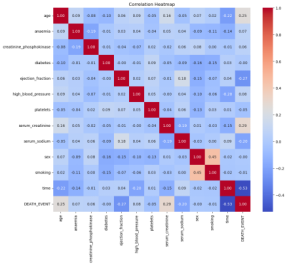
\includegraphics[width=0.5\linewidth]{image.png}
    \label{fig:placeholder}
\end{figure}

\textbf{Figure 1. Correlation heatmap of clinical variables.}

The analysis revealed that follow-up time (time) exhibited the strongest negative correlation with mortality (r = −0.53). In contrast, serum creatinine showed a moderate positive correlation (r = 0.29), whereas ejection fraction demonstrated a moderate negative correlation (r = −0.27). Although several additional variables showed weak associations with mortality, their correlation coefficients were considerably lower, suggesting relatively limited predictive value.

Overall, patients with shorter follow-up times tended to experience mortality more frequently. Higher serum creatinine levels were associated with increased mortality risk, whereas lower ejection fraction was associated with poorer survival outcomes.

It should be noted that Pearson correlation analysis evaluates only linear relationships and does not directly quantify the predictive contribution of individual variables. Therefore, additional statistical and machine learning analyses were performed to further assess predictor importance. 

\subsubsection{Mann–Whitney U Test}

Because several clinical variables were not normally distributed, the Mann–Whitney U test was performed to compare differences between the deceased and surviving patient groups.

Five variables demonstrated statistically significant differences (P < 0.05) between the two groups:

\textbf{Table 1. Results of the Mann–Whitney U test.}

\begin{table}[htbp]
\centering

\begin{tabular}{l l l}\toprule
Variable & U statistic & P value \\\midrule

Follow-up time & 16288.5 & \(6.85 \times 10^{-21}\)\\
Serum creatinine & 5298.0 & \(1.58 \times 10^{-10}\)\\
Ejection fraction & 13176.5 & \(7.37\times 10^{-7}\)\\
Age & 7121.0 & \(1.67 \times 10^{-4}\)\\
Serum sodium & 12261.5 & \(2.93 \times 10^{-4}\)\\ \bottomrule

\end{tabular}

\end{table}

Among these variables, follow-up time, serum creatinine, and ejection fraction exhibited the strongest statistical significance, consistent with the findings of the Pearson correlation analysis. Although age and serum sodium also showed statistically significant differences between groups, their overall contribution to prediction was comparatively lower when combined with subsequent machine learning analyses. Consequently, these variables were not selected as the final core predictors. 

\subsubsection{Random Forest Feature Importance Analysis}

To further evaluate the contribution of individual variables to mortality prediction, feature importance scores were calculated using the Random Forest model.
\begin{figure}[htbp]
    \centering
    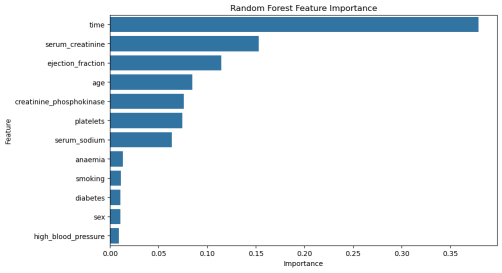
\includegraphics[width=0.5\linewidth]{image2.png}
    \label{fig:placeholder}
\end{figure}

\textbf{Figure 2. Feature importance ranking generated by the Random Forest model.}

The Random Forest algorithm ranked clinical variables according to their contribution to prediction during the tree construction process. Compared with conventional statistical analyses, this approach provides a more comprehensive evaluation of predictor importance by accounting for nonlinear relationships and complex interactions among variables.

By integrating the results of Pearson correlation analysis, the Mann–Whitney U test, and Random Forest feature importance analysis, three variables—follow-up time, serum creatinine, and ejection fraction—were consistently identified as the most informative predictors. These variables simultaneously demonstrated strong correlations with mortality, statistically significant differences between patient groups, and high importance scores within the Random Forest model.

Accordingly, these three variables were selected as the core predictors for subsequent model development.

The combination of statistical analysis and machine learning-based feature selection enhanced the robustness of predictor identification while reducing potential bias associated with any single analytical approach.

 
\subsection{Comparison of Machine Learning Models}

Following feature selection, four predictive models, namely Logistic Regression (LR), Random Forest (RF), eXtreme Gradient Boosting (XGBoost), and Multilayer Perceptron (MLP), were developed to predict mortality in patients with heart failure. Model performance was comprehensively evaluated using Accuracy, Precision, Recall, F1-score, and ROC-AUC.

\textbf{Table 2. Performance comparison of different machine learning models.}

\begin{table}[htbp]
\centering

\begin{tabular}{l l l l l l}\toprule
Model & Accuracy & Precision & Recall & F1-score & ROC-AUC \\\midrule

Logistic Regression & 0.817 & 0.786 & 0.579 & 0.667 & 0.859 \\
Random Forest & 0.817 & 0.786 & 0.579 & 0.667 & 0.883\\
XGBoost & 0.817 & 0.833 & 0.526 & 0.645 & 0.836 \\
MLP & 0.733 & 0.600 & 0.474 & 0.529 & 0.782 \\ \bottomrule

\end{tabular}

\end{table}

The comparative results demonstrated that the four models achieved relatively similar performance in terms of Accuracy, whereas more pronounced differences were observed for ROC-AUC, which reflects the discriminative ability of each classifier.

Among all evaluated models, the Random Forest algorithm achieved the highest ROC-AUC (0.883), indicating superior capability in distinguishing between patients who survived and those who experienced mortality during follow-up. Although Logistic Regression produced a relatively high ROC-AUC of 0.859, its overall discriminative performance remained slightly inferior to that of Random Forest. The XGBoost model achieved an ROC-AUC of 0.836, while the MLP model exhibited the lowest performance, with an ROC-AUC of 0.782.

To further compare the discriminative performance of the four models, receiver operating characteristic (ROC) curves were generated.
\begin{figure}[htbp]
    \centering
    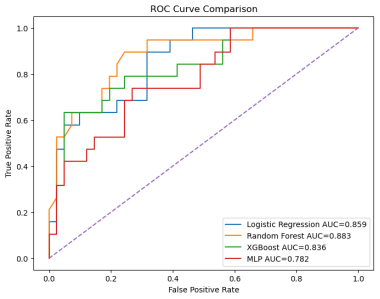
\includegraphics[width=0.5\linewidth]{image3.png}
    \label{fig:placeholder}
\end{figure}

\textbf{Figure 3. ROC curves of the four machine learning models.}

As illustrated in Figure 3, the ROC curve of the Random Forest model consistently remained above those of the other models across most decision thresholds and exhibited the largest area under the curve, further confirming its superior predictive performance.

Considering all evaluation metrics collectively, including Accuracy, Precision, Recall, F1-score, and ROC-AUC, the Random Forest model demonstrated the best overall predictive performance and was therefore selected as the optimal model for subsequent individualized mortality risk prediction. 

\subsection{Individualized Mortality Risk Prediction}

To further evaluate the practical applicability of the proposed prediction framework, the Random Forest model, which exhibited the best predictive performance, was applied to estimate the individualized mortality risk of a representative simulated patient.

The clinical characteristics of the simulated patient were as follows:

\begin{itemize}
    \item Age:75 years 
    \item Left ventricular ejection fraction:30\% 
    \item Serum creatinine:1.8 mg/dL 
    \item Follow-up time:50 days 
\end{itemize}
After these clinical variables were entered into the optimized Random Forest model, the predicted probability of mortality was 0.845, corresponding to an estimated mortality risk of 84.5\%.

Unlike conventional binary classification models that provide only categorical predictions (survival or death), the proposed model generated a continuous probability estimate that quantitatively reflected the patient's individual risk level. Such probability-based prediction enables more intuitive assessment of disease severity and facilitates comparison of mortality risk among different patients.

These findings demonstrate that the proposed Random Forest model not only achieved excellent overall predictive performance but also provided individualized probability estimates of mortality, highlighting its potential value as a clinical decision-support tool for personalized risk stratification and prognosis assessment in patients with heart failure.

 

\section{Discussion}

\subsection{Principal Findings}

The present study developed an individualized mortality risk prediction model for patients with heart failure by integrating conventional statistical analyses with multiple machine learning algorithms. Through systematic feature selection and comparative model evaluation, three clinical variables—follow-up time, serum creatinine, and left ventricular ejection fraction (LVEF)—were consistently identified as the most informative predictors of mortality. Among the four predictive models evaluated, the Random Forest algorithm achieved the best overall performance, with a ROC-AUC of 0.883, indicating excellent discriminative ability for mortality prediction.

Unlike traditional binary classification approaches that simply classify patients as survivors or non-survivors, the proposed model generated individualized mortality probabilities, allowing quantitative assessment of patient-specific risk. This probability-based prediction framework provides more clinically informative results and may facilitate personalized risk stratification and decision-making in routine clinical practice. 

\subsection{Clinical Significance of the Identified Predictors}

Feature selection demonstrated that follow-up time, serum creatinine, and left ventricular ejection fraction were consistently associated with mortality across Pearson correlation analysis, the Mann–Whitney U test, and Random Forest feature importance analysis.\cite{McDonagh2021,Heidenreich2022,Pocock2013}

Among these predictors, follow-up time exhibited the strongest association with mortality. Patients with shorter follow-up durations generally experienced poorer clinical outcomes, suggesting that disease progression during the early follow-up period may be closely associated with increased mortality risk.\cite{Cox1972}

Serum creatinine, an established indicator of renal function, was another important predictor identified in this study. Renal dysfunction is highly prevalent among patients with heart failure because of the close physiological interaction between the cardiovascular and renal systems. Elevated serum creatinine levels reflect impaired renal function and have been consistently associated with unfavorable prognosis in previous clinical studies.\cite{McDonagh2021,Damman2014}

Left ventricular ejection fraction (LVEF), a key indicator of cardiac systolic function, also demonstrated strong predictive value. Reduced LVEF reflects impaired myocardial contractility and diminished cardiac output, both of which are well-recognized indicators of disease severity and adverse clinical outcomes.\cite{McDonagh2021,Heidenreich2022}

Collectively, these three predictors capture complementary aspects of disease progression, renal function, and cardiac function, thereby providing a comprehensive representation of the clinical status of patients with heart failure. Their consistent identification across multiple analytical approaches further supports their importance in individualized mortality risk prediction. 

\subsection{Comparison of Machine Learning Models}

Among the four predictive models evaluated, Random Forest achieved the highest overall predictive performance, with a ROC-AUC of 0.883, outperforming Logistic Regression, XGBoost, and MLP.\cite{Rajkomar2019}

Random Forest is an ensemble learning algorithm that combines the predictions of multiple decision trees through bootstrap aggregation, thereby reducing variance and improving model robustness. Unlike conventional linear models, Random Forest effectively captures complex nonlinear relationships and interactions among clinical variables, making it particularly suitable for heterogeneous clinical datasets.\cite{Breiman2001}

Although Logistic Regression demonstrated satisfactory predictive performance and offers excellent interpretability, its underlying assumption of linear relationships between predictors and outcomes may limit its ability to model complex clinical data.\cite{Hosmer2013}

XGBoost, another ensemble learning algorithm, also demonstrated competitive predictive performance. However, its overall discriminative ability remained slightly lower than that of Random Forest in the present study, suggesting that Random Forest provided better adaptation to the characteristics of the current dataset.\cite{Chen2016}

The Multilayer Perceptron (MLP) exhibited the lowest predictive performance among the evaluated models. A possible explanation is the relatively limited sample size of the dataset. Neural network models generally require substantially larger training datasets to fully exploit their capacity for learning complex feature representations. Consequently, the potential advantages of deep learning were not fully realized in this study.\cite{Esteva2019,Goodfellow2016}

Overall, these findings indicate that machine learning algorithms are capable of effectively predicting mortality in patients with heart failure, with Random Forest providing the most favorable balance between predictive accuracy and model robustness under the current experimental conditions. 

\subsection{Clinical Implications}

With the growing emphasis on precision medicine, clinical decision-making has gradually shifted from experience-based judgment toward data-driven risk assessment. Accurate prediction of mortality risk in patients with heart failure not only facilitates early identification of high-risk individuals but also provides valuable information for treatment planning, follow-up management, and healthcare resource allocation.

The proposed prediction model integrates routinely available clinical variables and generates individualized mortality probabilities rather than simple binary predictions. Such probability-based risk estimates provide a more refined assessment of patient prognosis and may assist clinicians in implementing risk-stratified management strategies according to individual patient characteristics.

Furthermore, all predictors incorporated into the model are routinely collected during standard clinical practice and do not require additional laboratory tests or specialized examinations. Therefore, the proposed framework has favorable feasibility for clinical implementation and may serve as a practical decision-support tool. Nevertheless, the model is intended to complement, rather than replace, clinical judgment. Final clinical decisions should always be made by healthcare professionals based on comprehensive evaluation of patient history, physical examination findings, imaging studies, and other relevant clinical information.

 
\subsection{Study Limitations}

Despite the promising findings, several limitations of the present study should be acknowledged.

First, the proposed prediction model was developed and validated using a publicly available heart failure dataset with a relatively limited sample size. Although this dataset has been widely adopted in machine learning research, its relatively small number of participants and single-source origin may restrict the generalizability of the proposed model. Therefore, further validation using larger and more diverse patient cohorts is warranted.

Second, the present study relied exclusively on routinely collected clinical variables. Other potentially informative data sources, including medical imaging, genomic information, proteomic profiles, and novel circulating biomarkers, were not incorporated into the prediction model. Integration of these multimodal data may further improve predictive performance and provide a more comprehensive representation of disease progression.

Third, only four machine learning algorithms—Logistic Regression, Random Forest, XGBoost, and Multilayer Perceptron—were evaluated. Although these models represent widely used approaches in clinical prediction research, recently developed algorithms, such as transformer-based architectures, graph neural networks, and advanced ensemble learning methods, were beyond the scope of this study. Future investigations may explore these techniques to further enhance predictive accuracy.

Finally, external validation using independent real-world datasets was not performed. Consequently, the robustness and clinical applicability of the proposed model across different healthcare settings and patient populations remain to be established. Prospective multicenter validation studies are therefore necessary before the model can be considered for routine clinical implementation. 

\subsection{Future Perspectives}

Future studies should focus on expanding the sample size by integrating multicenter clinical datasets from different healthcare institutions to improve both the generalizability and robustness of prediction models.

In addition, incorporating multimodal medical data—including imaging, genomics, wearable-device data, and longitudinal electronic health records—may enable more comprehensive characterization of disease progression and further improve individualized risk prediction.

Another important direction involves enhancing model interpretability. Although machine learning algorithms have demonstrated excellent predictive performance, their clinical adoption depends not only on predictive accuracy but also on transparency and explainability. Future studies may integrate interpretable artificial intelligence techniques, such as SHAP (SHapley Additive exPlanations) or LIME (Local Interpretable Model-agnostic Explanations), to quantify the contribution of individual clinical variables and improve clinicians' confidence in model-assisted decision-making.

Furthermore, prospective validation in real-world clinical environments should be conducted to evaluate the effectiveness, reliability, and clinical utility of the proposed framework. Successful integration of machine learning models into hospital information systems and clinical decision-support platforms may facilitate precision medicine and contribute to more personalized management of patients with heart failure. 

 

\section{Conclusion}
In this study, a machine learning-based mortality risk prediction model integrating clinical indicators was developed for patients with heart failure using a combination of statistical analyses and machine learning techniques. Comprehensive feature selection identified follow-up time, serum creatinine, and left ventricular ejection fraction as the most informative predictors associated with mortality.

Among the four evaluated machine learning algorithms, Random Forest achieved the best overall predictive performance, with a ROC-AUC of 0.883, outperforming Logistic Regression, XGBoost, and Multilayer Perceptron. Furthermore, the optimized Random Forest model successfully generated individualized mortality probabilities, extending conventional binary classification to quantitative probability-based risk assessment.

Overall, the proposed framework demonstrates that integrating routinely available clinical indicators with machine learning algorithms provides an effective approach for individualized mortality prediction in patients with heart failure. The model has the potential to support clinical risk stratification and personalized decision-making while contributing to the ongoing development of precision medicine.

Nevertheless, additional multicenter studies with larger patient populations and external validation are required before widespread clinical implementation. Future integration of multimodal medical data and interpretable artificial intelligence techniques may further improve predictive performance and facilitate translation of the proposed framework into routine clinical practice. 

 \bibliographystyle{unsrt}
\bibliography{references}


\end{document}